\chapter{Propozycja klasyfikatorów}
\section{Klasyfikator ekspercki}
Klasyfikator ekspercki powstał na bazie doświadczeń z podstawowymi klasyfikatorami. W zależności od charakterystyki danych, osiągana skuteczność przez klasyfikatory może się różnić. Klasyfikator skutecznie rozpoznający klasy jednego zbioru może miernie klasyfikować inny zbiór, podczas gdy użycie innego klasyfikatora na tym samym zbiorze danych może znacząco poprawić osiągane wyniki. Również użycie różnych algorytmów klasyfikacji, połączenie ich w komitet może zmniejszyć błąd klasyfikacji. 
Klasyfikator ekspercki został stworzony w celu zmniejszenia błędu klasyfikacji, niezależnie od typu danych oraz nieznanych danych. \par
Klasyfikator ekspercki to połączenie kilku klasyfikatorów (przynajmniej trzech), najlepiej z różnymi algorytmami lub ustawieniami. Każdy klasyfikator trenowany jest na zbiorze uczącym, a następnie oceniana jest jakość klasyfikacji każdego z osobna. Stworzono dwie wersje klasyfikatora, w pierwszej klasyfikator uczony i testowany jest na tym samym zbiorze danych, w drugiej oceniany jest z wykorzystaniem sprawdzianu krzyżowego (domyślnie k=3). W kolejnym etapie, dla każdej klasy wyłaniany jest klasyfikator ekspert. Ekspert klasowy wybierany jest na podstawie najwyższego współczynnika dla danej klasy. Tworząc klasyfikator można wybrać na podstawie którego współczynnika precyzji, F1 czy G-mean będą wyłaniani eksperci. Domyślnie jest to współczynnik precyzji. Przy wyborze miary G-mean ekspert dla obu będzie taki sam. Jeżeli ocena odbywała się ze sprawdzianem krzyżowym, to modele klasyfikatora tworzone są od nowa, na całym zbiorze treningowym. \par
W procesie klasyfikacji właściwej, nowe próbki klasyfikowane są najpierw przez klasyfikatory składowe. Końcowa klasa wyznaczana jest według algorytmu:
\begin{enumerate}
	\item Jeżeli występuje zgodność co do klasy pomiędzy klasyfikatorami, to wybierana jest ta klasa.
	\item Jeżeli tylko jeden ekspert wskaże swoją klasę, to ostateczną klasą jest ta wskazana przez eksperta.
	\item Jeżeli dwóch ekspertów wskaże swoje klasy, to wybierana jest klasa z większym prawdopodobieństwem wskazanym przez klasyfikator. W przypadku takich samych prawdopodobieństw, wybierana jest klasa wskazana przez klasyfikator z większym współczynnikiem G-mean.
	\item Jeżeli żaden ekspert nie wskaże swojej klasy, to klasa wybierana jest poprzez głosowanie większościowe.
\end{enumerate}
\begin{figure}[H]
	\centering
	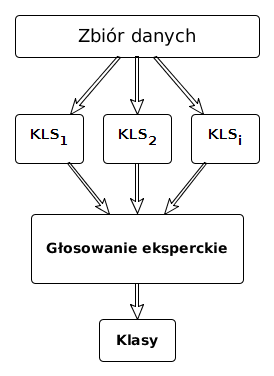
\includegraphics[width=0.3\textwidth]{./images/klas_ekspercki.png}
	\caption{Schemat klasyfikatora eksperckiego. $KLS_1..KLS_i$ to klasyfikatory składowe.}
	\label{fig:klasyfikator_ekspercki}
\end{figure}
Podstawowa wersja klasyfikatora znajduje się w pliku $classifiers/clf\_expert.py$, a wersja ze sprawdzianem krzyżowym w pliku $classifiers/clf\_expertCV.py$. Obsługa klasyfikatora odbywa się w takim sam sposób jak klasyfikatorów z biblioteki $scikit-learn$.
\subsection{Test klasyfikatora eksperckiego}
Test klasyfikatora eksperckiego przeprowadzono tak samo jak poprzednie. Został on powtórzony 10 razy, a wyniki zostały uśrednione. Test znajduje się w pliku $test\_my\_clfs/test\_clf\_expert.py$. Klasyfikator ekspercki został zbudowany z naiwnego klasyfikatora Bayesa, klasyfikatora kNN oraz drzewa decyzyjnego z maksymalną głębokością 3. Test przeprowadzono dla różnych funkcji wyłaniających ekspertów. CLFE to podstawowa wersja klasyfikatora, eksperci klasowi wyłaniani są na podstawie najlepszej precyzji. W CLFE F1 eksperci wyłaniani są na podstawie miary F-1 klas. Natomiast w CLFE G wyłonienie ekspertów odbywa się na podstawie miary G-mean. Skrót CV, oznacza wersję ze sprawdzianem krzyżowym. Wyniki zostały porównane do drzewa decyzyjnego (TREE) z maksymalną głębokością równą 3. Dokładność klasyfikacji (tabela \ref{ekspertacc}) oraz czułość klasy większościowej (tabela \ref{ekspertsens}) wzrosła dla większości zbiorów danych. Dla pozostałych zbiorów, wyniki były takie same jak drzewa decyzyjnego lub minimalnie niższe. Natomiast specyficzność klasy mniejszościowej (tabela \ref{ekspertspec}) oraz miara G-mean (tabela \ref{ekspertgmean}) wzrosły lub utrzymały taką samą wartości jak drzewa decyzyjne w 21 zbiorach na 22. W wykrywaniu klasy mniejszościowej najlepsze okazały się klasyfikatory oparty o miarę F1 i G-mean. Pomiędzy wersją klasyfikatora ze sprawdzianem krzyżowym oraz bez, nie zauważono dużej różnicy w wynikach w większości zbiorów.
	\begin{table}[H]
		\tiny
		\begin{center}
			\resizebox{\textwidth}{!}{%
				\begin{tabular}{c|ccccccc}%
					Zbiór danych&TREE&CLFE&CLFE CV&CLFE F1&\specialcell{CLFE\\F1 CV}&CLFE G&\specialcell{CLFE\\G CV}\\%
					\hline%
					seeds&0.91&\textbf{0.92}&0.91&0.91&0.91&0.91&0.91\\%
					new\_thyroid&\textbf{0.97}&\textbf{0.97}&\textbf{0.97}&\textbf{0.97}&0.96&\textbf{0.97}&0.96\\%
					vehicle&0.9&0.9&0.9&\textbf{0.92}&\textbf{0.92}&\textbf{0.92}&0.9\\%
					ionosphere&0.86&0.88&\textbf{0.89}&0.86&0.87&0.86&0.87\\%
					vertebal&0.71&0.74&0.73&0.73&0.77&0.73&\textbf{0.78}\\%
					yeastME3&0.94&\textbf{0.95}&\textbf{0.95}&\textbf{0.95}&0.94&\textbf{0.95}&0.94\\%
					ecoli&0.86&0.85&0.85&0.87&0.87&\textbf{0.88}&0.76\\%
					bupa&0.65&\textbf{0.69}&0.68&0.68&0.67&0.68&0.6\\%
					horse\_colic&\textbf{0.86}&\textbf{0.86}&0.84&\textbf{0.86}&\textbf{0.86}&\textbf{0.86}&\textbf{0.86}\\%
					german&0.74&\textbf{0.76}&0.75&0.73&\textbf{0.76}&0.73&0.74\\%
					breast\_cancer&\textbf{0.73}&0.71&0.71&0.7&0.72&0.72&0.72\\%
					cmc&\textbf{0.78}&0.75&0.76&0.74&0.74&0.7&0.68\\%
					hepatitis&0.66&\textbf{0.68}&\textbf{0.68}&0.66&0.66&0.61&0.66\\%
					haberman&\textbf{0.75}&0.73&0.74&0.74&0.74&0.74&0.69\\%
					transfusion&0.68&\textbf{0.69}&0.68&0.68&\textbf{0.69}&0.68&\textbf{0.69}\\%
					car&0.69&0.89&\textbf{0.92}&\textbf{0.92}&\textbf{0.92}&0.89&0.89\\%
					glass&\textbf{0.82}&0.63&0.8&\textbf{0.82}&0.74&0.49&0.48\\%
					abalone16\_29&\textbf{0.94}&\textbf{0.94}&\textbf{0.94}&0.93&0.88&0.68&0.68\\%
					solar\_flare&\textbf{0.95}&0.81&0.94&\textbf{0.95}&0.87&0.65&0.65\\%
					heart\_cleveland&\textbf{0.86}&\textbf{0.86}&0.83&0.85&0.83&0.81&0.81\\%
					balance\_scale&\textbf{0.92}&\textbf{0.92}&\textbf{0.92}&\textbf{0.92}&\textbf{0.92}&\textbf{0.92}&\textbf{0.92}\\%
					postoperative&0.68&0.69&0.71&0.67&\textbf{0.72}&0.67&0.67\\%
				\end{tabular}}
				\caption{Dokładność klasyfikatora eksperckiego.}
				\label{ekspertacc}
			\end{center}
		\end{table}	
			\begin{table}[H]
				\tiny
				\begin{center}
					\resizebox{\textwidth}{!}{%
						\begin{tabular}{c|ccccccc}%
							Zbiór danych&TREE&CLFE&CLFE CV&CLFE F1&\specialcell{CLFE\\F1 CV}&CLFE G&\specialcell{CLFE\\G CV}\\%
							\hline%
							seeds&\textbf{0.92}&\textbf{0.92}&0.91&\textbf{0.92}&\textbf{0.92}&\textbf{0.92}&\textbf{0.92}\\%
							new\_thyroid&0.98&0.98&\textbf{0.99}&0.98&\textbf{0.99}&0.98&0.97\\%
							vehicle&0.89&0.89&0.89&\textbf{0.95}&\textbf{0.95}&\textbf{0.95}&0.89\\%
							ionosphere&0.92&0.97&\textbf{0.99}&0.92&0.93&0.92&0.93\\%
							vertebal&0.71&\textbf{0.72}&0.71&0.71&0.71&0.71&\textbf{0.72}\\%
							yeastME3&0.97&0.97&0.97&\textbf{0.98}&0.97&0.97&0.97\\%
							ecoli&0.9&0.88&0.86&\textbf{0.91}&0.89&0.9&0.77\\%
							bupa&0.72&0.77&0.81&0.81&0.72&\textbf{0.82}&0.63\\%
							horse\_colic&\textbf{0.92}&\textbf{0.92}&0.88&\textbf{0.92}&\textbf{0.92}&\textbf{0.92}&\textbf{0.92}\\%
							german&0.88&\textbf{0.89}&\textbf{0.89}&0.86&0.84&0.77&0.81\\%
							breast\_cancer&\textbf{0.92}&0.88&0.85&0.85&0.86&0.84&0.84\\%
							cmc&\textbf{0.9}&0.86&0.86&0.88&0.83&0.75&0.7\\%
							hepatitis&0.7&\textbf{0.73}&\textbf{0.73}&0.7&0.67&0.59&0.63\\%
							haberman&0.91&0.91&\textbf{0.93}&0.9&\textbf{0.93}&0.88&0.85\\%
							transfusion&0.76&\textbf{0.81}&0.8&0.8&\textbf{0.81}&0.76&0.8\\%
							car&0.71&0.89&\textbf{0.94}&\textbf{0.94}&\textbf{0.94}&0.89&0.89\\%
							glass&\textbf{0.88}&0.64&0.85&\textbf{0.88}&0.78&0.48&0.45\\%
							abalone16\_29&\textbf{1.0}&0.99&0.99&0.99&0.92&0.69&0.69\\%
							solar\_flare&\textbf{0.99}&0.83&0.98&0.98&0.88&0.64&0.64\\%
							heart\_cleveland&\textbf{0.97}&\textbf{0.97}&0.89&0.91&0.89&0.83&0.83\\%
							balance\_scale&\textbf{1.0}&\textbf{1.0}&\textbf{1.0}&\textbf{1.0}&\textbf{1.0}&\textbf{1.0}&\textbf{1.0}\\%
							postoperative&0.9&0.89&0.94&0.83&\textbf{0.95}&0.83&0.85\\%
						\end{tabular}}
						\caption{Czułość klasy większościowej dla klasyfikatora eksperckiego.}
						\label{ekspertsens}
					\end{center}
				\end{table}	
			\begin{table}[H]
				\tiny
				\begin{center}
					\resizebox{\textwidth}{!}{%
						\begin{tabular}{c|ccccccc}%
							Zbiór danych&TREE&CLFE&CLFE CV&CLFE F1&\specialcell{CLFE\\F1 CV}&CLFE G&\specialcell{CLFE\\G CV}\\%
							\hline%
							seeds&0.89&\textbf{0.91}&0.9&0.89&0.9&0.89&0.9\\%
							new\_thyroid&\textbf{0.87}&\textbf{0.87}&0.8&\textbf{0.87}&0.8&\textbf{0.87}&\textbf{0.87}\\%
							vehicle&\textbf{0.93}&\textbf{0.93}&\textbf{0.93}&0.84&0.84&0.84&\textbf{0.93}\\%
							ionosphere&0.75&0.71&0.71&0.75&\textbf{0.76}&0.75&\textbf{0.76}\\%
							vertebal&0.71&0.76&0.76&0.76&\textbf{0.9}&0.76&\textbf{0.9}\\%
							yeastME3&0.73&\textbf{0.77}&\textbf{0.77}&0.71&0.7&0.75&0.73\\%
							ecoli&0.49&0.6&0.71&0.51&0.63&\textbf{0.74}&0.69\\%
							bupa&0.55&0.57&0.5&0.5&\textbf{0.61}&0.48&0.57\\%
							horse\_colic&0.75&0.75&\textbf{0.78}&0.75&0.76&0.75&0.76\\%
							german&0.42&0.46&0.44&0.44&0.55&\textbf{0.62}&0.57\\%
							breast\_cancer&0.31&0.31&0.39&0.35&0.41&0.42&\textbf{0.44}\\%
							cmc&0.39&0.37&0.42&0.28&0.45&0.51&\textbf{0.61}\\%
							hepatitis&0.5&0.5&0.5&0.5&0.62&0.69&\textbf{0.78}\\%
							haberman&0.32&0.23&0.21&0.28&0.2&\textbf{0.35}&0.25\\%
							transfusion&\textbf{0.45}&0.32&0.3&0.31&0.3&0.41&0.35\\%
							car&0.32&\textbf{1.0}&0.43&0.43&0.43&\textbf{1.0}&\textbf{1.0}\\%
							glass&0.12&0.47&0.24&0.12&0.29&0.65&\textbf{0.82}\\%
							abalone16\_29&0.09&0.13&0.15&0.13&0.28&\textbf{0.58}&\textbf{0.58}\\%
							solar\_flare&0.12&0.44&0.12&0.09&0.63&\textbf{0.93}&\textbf{0.93}\\%
							heart\_cleveland&0.03&0.03&0.34&0.37&0.31&\textbf{0.63}&\textbf{0.63}\\%
							balance\_scale&\textbf{0.0}&\textbf{0.0}&\textbf{0.0}&\textbf{0.0}&\textbf{0.0}&\textbf{0.0}&\textbf{0.0}\\%
							postoperative&0.08&0.12&0.08&\textbf{0.21}&0.08&\textbf{0.21}&0.17\\%
						\end{tabular}}
						\caption{Specyficzność klasy mniejszościowej dla klasyfikatora eksperckiego.}
						\label{ekspertspec}
					\end{center}
				\end{table}	
			\begin{table}[H]
				\tiny
				\begin{center}
					\resizebox{\textwidth}{!}{%
						\begin{tabular}{c|ccccccc}%
							Zbiór danych&TREE&CLFE&CLFE CV&CLFE F1&\specialcell{CLFE\\F1 CV}&CLFE G&\specialcell{CLFE\\G CV}\\%
							\hline%
							seeds&0.9&\textbf{0.92}&0.91&0.9&0.91&0.9&0.91\\%
							new\_thyroid&\textbf{0.92}&\textbf{0.92}&0.89&\textbf{0.92}&0.89&\textbf{0.92}&\textbf{0.92}\\%
							vehicle&\textbf{0.91}&\textbf{0.91}&\textbf{0.91}&0.89&0.89&0.89&\textbf{0.91}\\%
							ionosphere&0.83&0.83&\textbf{0.84}&0.83&\textbf{0.84}&0.83&\textbf{0.84}\\%
							vertebal&0.71&0.74&0.74&0.74&\textbf{0.8}&0.74&\textbf{0.8}\\%
							yeastME3&0.84&\textbf{0.86}&\textbf{0.86}&0.83&0.82&0.85&0.84\\%
							ecoli&0.66&0.73&0.79&0.69&0.75&\textbf{0.82}&0.73\\%
							bupa&0.63&\textbf{0.67}&0.64&0.63&0.66&0.63&0.6\\%
							horse\_colic&\textbf{0.83}&\textbf{0.83}&\textbf{0.83}&\textbf{0.83}&\textbf{0.83}&\textbf{0.83}&\textbf{0.83}\\%
							german&0.61&0.64&0.63&0.61&0.68&\textbf{0.69}&0.68\\%
							breast\_cancer&0.53&0.52&0.57&0.55&0.59&\textbf{0.6}&\textbf{0.6}\\%
							cmc&0.59&0.56&0.6&0.49&0.61&0.62&\textbf{0.65}\\%
							hepatitis&0.59&0.6&0.6&0.59&0.65&0.63&\textbf{0.7}\\%
							haberman&0.54&0.46&0.44&0.5&0.43&\textbf{0.55}&0.46\\%
							transfusion&\textbf{0.59}&0.51&0.49&0.5&0.49&0.56&0.53\\%
							car&0.48&\textbf{0.94}&0.64&0.63&0.63&\textbf{0.94}&\textbf{0.94}\\%
							glass&0.32&0.55&0.45&0.32&0.48&0.56&\textbf{0.61}\\%
							abalone16\_29&0.3&0.35&0.39&0.35&0.5&\textbf{0.63}&\textbf{0.63}\\%
							solar\_flare&0.34&0.61&0.34&0.3&0.74&\textbf{0.77}&\textbf{0.77}\\%
							heart\_cleveland&0.17&0.17&0.55&0.58&0.53&\textbf{0.72}&\textbf{0.72}\\%
							balance\_scale&\textbf{0.0}&\textbf{0.0}&\textbf{0.0}&\textbf{0.0}&\textbf{0.0}&\textbf{0.0}&\textbf{0.0}\\%
							postoperative&0.27&0.33&0.28&\textbf{0.42}&0.28&\textbf{0.42}&0.38\\%
						\end{tabular}}
						\caption{Miara G-mean dla klasyfikatora eksperckiego.}
						\label{ekspertgmean}
					\end{center}
				\end{table}	
\section{Meta-klasyfikator}
Algorytm klasyfikacji danych wybiera się w zależności od charakterystyki i rodzaju danych. Budowany meta-klasyfikator miał osiągać dobre wyniki dla różnych zbiorów danych. Architektura zbudowanego meta-klasyfikatora jest bardzo złożona. Została przedstawiona na rysunku \ref{fig:metaklasmoj}. W pierwszej warstwie składa się on z klasyfikatora eksperckiego oraz z kilku klasyfikatorów bagging, boosting oraz stacking. Tworząc meta-klasyfikator należy wybrać z jakich klasyfikatorów utworzone będą klasyfikatory bagging, boosting, stacking oraz klasyfikator ekspercki. Można wybrać kilka klasyfikatorów do utworzenia kilku klasyfikatorów bagging oraz boosting. Klasyfikatorami składowymi mogą być różne algorytmy klasyfikacji lub takie same algorytmy ale innymi ustawieniami. Klasyfikator ekspercki oraz stacking tworzone są z tych samych klasyfikatorów składowych. W kolejnym kroku oceniany jest każdy model klasyfikacyjny poprzez sprawdzian krzyżowy dla niemodyfikowanego zbioru danych, dla zmodyfikowanego metodą NCR oraz dla zmodyfikowanego metodą SMOTE. Każda instancja klasyfikatora jest najpierw kopiowana, a następnie uczona na kolejnym zbiorze danych. Do końcowej klasyfikacji wybierane są trzy najlepsze klasyfikatory ze zbiorami danych, dla których osiągnęły najlepszy wynik. Kryterium wyboru najlepszych klasyfikatorów stanowi miara G-mean. W ostatnim etapie wybrane klasyfikatory trenowane są na pełnym zbiorze danych, a następnie klasyfikują ten zbiór danych, tworząc meta-dane stanowiące zbiór uczący dla końcowego meta-klasyfikatora - sieci neuronowej wielowarstwowej. Ostateczną klasę klasyfikowanemu przykładowi nadaje sieć neuronowa. Kod klasyfikatora znajduje się w pliku $classifiers/meta\_clf.py$.
\begin{figure}[H]
	\centering
	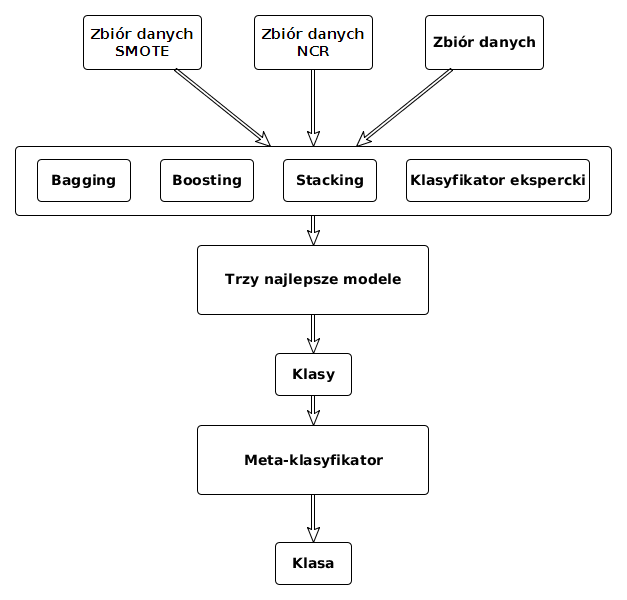
\includegraphics[width=0.7\textwidth]{./images/metaklas.png}
	\caption{Projekt meta-klasyfikatora}
	\label{fig:metaklasmoj}
\end{figure}
\subsection{Testy}
Do stworzenia testowego meta-klasyfikatora wybrano klasyfikator kNN, drzewo decyzyjne z maksymalną głębokością 3 oraz naiwny klasyfikator Bayesa. Z tych trzech klasyfikatorów utworzono klasyfikator ekspercki, stacking oraz trzy modele klasyfikacyjne bagging. Utworzono również dwa modele AdaBoost z drzewa decyzyjnego z maksymalną głębokością 3 oraz z naiwnego klasyfikatora Bayesa (klasyfikator kNN nie wspiera wag). Każdy utworzony klasyfikator składowy został przetestowany dla zbioru danych bez modyfikacji, dla zbioru zmodyfikowanego metodą NCR oraz dla zbioru zmodyfikowanego metodą SMOTE. Przy takiej konstrukcji, może wystąpić przypadek wyboru np. trzech modeli (kopii) tego samego klasyfikatora bagging zbudowanych dla różnych zbiorów danych. Przeprowadzony test znajduje się w pliku $test\_my\_clfs/test\_meta\_clf.py$. Otrzymane wyniki porównano do meta-metod oraz klasyfikatora eksperckiego, czyli klasyfikatorów wchodzących w skład meta-klasyfikatora. W tabeli \ref{metamyacc} przedstawiono dokładność, a w tabeli \ref{metamysens} czułość klasy większościowej meta-klasyfikatora. Nie udało uzyskać się najlepszego wyniku dla każdego zbioru, ale otrzymane wyniki zdecydowanie plasują się w czołówce. Jednocześnie udało się uniknąć i utrzymać wysoką jakość klasyfikacji dla wszystkich baz (np. klasyfikator bagging NKB, mimo wysokich wyników, dla $yeastME3$ uzyskał tylko 26\% dokładności). Jeżeli chodzi o rozpoznawalność klasy mniejszościowej (tabela specyficzności \ref{metamyacc}) oraz miarę G-mean (tabela \ref{metamygmean}) to otrzymane wyniki są powyżej średniej. Również tutaj udało uniknąć się bardzo niskich wyników jakie zdarzały się pojedynczym klasyfikatorom np. klasyfikator bagging kNN miał bardzo niską rozpoznawalność klasy mniejszościowej w bazie $german$, $breast\; cancer$, $hepatitis$, $glass$, $heart\; cleveland$. Natomiast meta-klasyfikator uzyskał wyniki plasujące go w czołówce dla wszystkich zbiorów danych. \par
Stworzony projekt meta-klasyfikatora stanowi interesującą propozycję uniwersalnego klasyfikatora. Skuteczność meta-klasyfikatora można poprawić poprzez zastosowanie bardziej różnorodnych algorytmów klasyfikacyjnych (np. można dodatkowo zastosować sieć neuronową) lub bardziej zaawansowanych metod równoważenia zbiorów danych.
\begin{table}[H]
	\tiny
	\begin{center}
		\resizebox{\textwidth}{!}{%
			\begin{tabular}{c|ccccccc}%
				Zbiór danych&\specialcell{Bag\\kNN}&\specialcell{Bag\\TREE}&\specialcell{Bag\\NKB}&\specialcell{Ada\\TREE}&\specialcell{Ada\\NKB}&CLFE&\specialcell{META}\\%
				\hline
				seeds&\textbf{0.83}&0.79&0.8&0.79&0.79&0.79&0.8\\%
				new\_thyroid&0.96&\textbf{0.97}&0.96&\textbf{0.97}&0.95&\textbf{0.97}&\textbf{0.97}\\%
				vehicle&0.93&0.91&0.67&\textbf{0.98}&0.85&0.93&0.97\\%
				ionosphere&0.77&\textbf{0.89}&0.86&0.86&\textbf{0.89}&0.84&0.85\\%
				vertebal&0.72&0.72&\textbf{0.78}&0.72&0.73&0.68&0.74\\%
				yeastME3&\textbf{0.95}&\textbf{0.95}&0.26&0.94&0.79&0.78&\textbf{0.95}\\%
				ecoli&0.84&0.81&0.84&\textbf{0.87}&0.43&0.8&0.78\\%
				bupa&\textbf{0.69}&0.65&0.55&0.67&0.58&0.6&0.65\\%
				horse\_colic&0.72&\textbf{0.85}&0.77&0.82&0.72&0.77&0.8\\%
				german&0.7&\textbf{0.76}&0.72&0.72&0.62&0.68&0.74\\%
				breast\_cancer&0.66&\textbf{0.73}&0.72&0.68&0.51&0.69&0.64\\%
				cmc&0.77&\textbf{0.79}&0.68&0.73&0.63&0.7&0.74\\%
				hepatitis&0.71&0.75&0.68&\textbf{0.81}&0.72&0.61&0.77\\%
				haberman&0.63&0.57&\textbf{0.72}&0.68&0.52&0.48&0.6\\%
				transfusion&0.72&\textbf{0.76}&0.74&0.64&0.59&0.65&0.58\\%
				car&0.97&0.95&0.89&\textbf{0.99}&0.96&0.89&0.97\\%
				glass&0.82&0.75&0.6&0.8&\textbf{0.87}&0.51&0.79\\%
				abalone16\_29&\textbf{0.94}&\textbf{0.94}&0.68&0.92&0.61&0.91&0.9\\%
				solar\_flare&\textbf{0.95}&\textbf{0.95}&0.67&0.93&0.58&0.94&0.94\\%
				heart\_cleveland&\textbf{0.88}&\textbf{0.88}&0.82&0.86&0.78&0.85&0.82\\%
				balance\_scale&\textbf{0.92}&\textbf{0.92}&\textbf{0.92}&0.87&\textbf{0.92}&0.81&0.85\\%
				postoperative&0.62&0.67&0.62&0.57&\textbf{0.7}&0.57&0.64\\%
			\end{tabular}}
			\caption{Dokładność meta-klasyfikatora.}
			\label{metamyacc}
		\end{center}
	\end{table}
	
\begin{table}[H]
	\tiny
	\begin{center}
		\resizebox{\textwidth}{!}{%
			\begin{tabular}{c|ccccccc}%
				Zbiór danych&\specialcell{Bag\\kNN}&\specialcell{Bag\\TREE}&\specialcell{Bag\\NKB}&\specialcell{Ada\\TREE}&\specialcell{Ada\\NKB}&CLFE&\specialcell{META}\\%
				\hline
				seeds&\textbf{0.79}&0.74&0.74&0.74&0.73&0.73&0.73\\%
				new\_thyroid&\textbf{1.0}&0.98&0.98&0.98&0.97&0.98&0.99\\%
				vehicle&0.95&0.92&0.62&\textbf{0.98}&0.91&0.96&0.97\\%
				ionosphere&\textbf{0.99}&0.92&0.88&0.88&0.96&0.86&0.87\\%
				vertebal&0.71&0.72&\textbf{0.73}&0.71&0.67&0.63&0.72\\%
				yeastME3&\textbf{0.98}&0.97&0.17&0.97&0.87&0.78&0.97\\%
				ecoli&0.87&0.84&0.83&\textbf{0.91}&0.37&0.78&0.8\\%
				bupa&\textbf{0.81}&0.76&0.38&0.74&0.74&0.57&0.59\\%
				horse\_colic&0.8&\textbf{0.91}&0.79&0.88&0.81&0.81&0.83\\%
				german&0.87&\textbf{0.92}&0.75&0.83&0.76&0.76&0.84\\%
				breast\_cancer&0.88&\textbf{0.92}&0.84&0.75&0.41&0.8&0.7\\%
				cmc&0.91&\textbf{0.93}&0.7&0.84&0.74&0.79&0.85\\%
				hepatitis&\textbf{0.89}&0.8&0.65&0.87&0.81&0.59&0.87\\%
				haberman&0.65&0.54&\textbf{0.89}&0.77&0.45&0.39&0.62\\%
				transfusion&0.86&0.91&\textbf{0.92}&0.75&0.68&0.76&0.67\\%
				car&\textbf{0.99}&0.98&0.89&\textbf{0.99}&0.97&0.88&0.98\\%
				glass&0.88&0.81&0.59&0.85&\textbf{0.94}&0.48&0.85\\%
				abalone16\_29&0.99&\textbf{1.0}&0.68&0.96&0.63&0.95&0.94\\%
				solar\_flare&\textbf{0.99}&\textbf{0.99}&0.66&0.97&0.59&0.97&0.97\\%
				heart\_cleveland&\textbf{1.0}&0.99&0.86&0.97&0.85&0.93&0.89\\%
				balance\_scale&\textbf{1.0}&\textbf{1.0}&\textbf{1.0}&0.94&\textbf{1.0}&0.88&0.92\\%
				postoperative&0.82&0.88&0.8&0.71&\textbf{0.94}&0.68&0.83\\%
			\end{tabular}}
			\caption{Czułość klasy większościowej meta-klasyfikatora.}
			\label{metamysens}
		\end{center}
	\end{table}
	
\begin{table}[H]
	\tiny
	\begin{center}
		\resizebox{\textwidth}{!}{%
			\begin{tabular}{c|ccccccc}%
				Zbiór danych&\specialcell{Bag\\kNN}&\specialcell{Bag\\TREE}&\specialcell{Bag\\NKB}&\specialcell{Ada\\TREE}&\specialcell{Ada\\NKB}&CLFE&\specialcell{META}\\%
				\hline
				seeds&0.93&0.87&0.93&0.89&0.91&0.9&\textbf{0.94}\\%
				new\_thyroid&0.73&\textbf{0.87}&\textbf{0.87}&\textbf{0.87}&\textbf{0.87}&\textbf{0.87}&0.83\\%
				vehicle&0.87&0.89&0.84&\textbf{0.95}&0.64&0.84&\textbf{0.95}\\%
				ionosphere&0.4&\textbf{0.83}&\textbf{0.83}&\textbf{0.83}&0.76&0.8&\textbf{0.83}\\%
				vertebal&0.73&0.72&\textbf{0.88}&0.75&0.84&0.78&0.79\\%
				yeastME3&0.69&0.8&\textbf{0.99}&0.69&0.21&0.77&0.8\\%
				ecoli&0.57&0.6&0.94&0.51&\textbf{0.97}&0.94&0.6\\%
				bupa&0.52&0.49&\textbf{0.79}&0.57&0.35&0.63&0.73\\%
				horse\_colic&0.59&\textbf{0.75}&0.74&0.73&0.58&0.71&\textbf{0.75}\\%
				german&0.3&0.37&\textbf{0.66}&0.46&0.3&0.49&0.5\\%
				breast\_cancer&0.16&0.28&0.44&0.51&\textbf{0.74}&0.42&0.51\\%
				cmc&0.27&0.28&\textbf{0.61}&0.32&0.26&0.36&0.34\\%
				hepatitis&0.03&0.53&\textbf{0.78}&0.59&0.34&0.72&0.38\\%
				haberman&0.57&0.67&0.25&0.41&0.69&\textbf{0.73}&0.53\\%
				transfusion&0.25&0.27&0.18&0.28&0.29&\textbf{0.31}&\textbf{0.31}\\%
				car&0.58&0.11&\textbf{1.0}&\textbf{1.0}&0.78&\textbf{1.0}&0.65\\%
				glass&0.06&0.12&0.71&0.24&0.12&\textbf{0.82}&0.12\\%
				abalone16\_29&0.11&0.07&\textbf{0.58}&0.28&0.31&0.3&0.4\\%
				solar\_flare&0.0&0.02&\textbf{0.93}&0.12&0.28&0.14&0.21\\%
				heart\_cleveland&0.0&0.06&\textbf{0.51}&0.06&0.23&0.31&0.26\\%
				balance\_scale&0.0&0.0&0.0&\textbf{0.08}&0.0&\textbf{0.08}&0.06\\%
				postoperative&0.08&0.08&0.12&0.17&0.04&\textbf{0.25}&0.12\\%
			\end{tabular}}
			\caption{Specyficzność klasy mniejszościowej meta-klasyfikatora.}
			\label{metamyspec}
		\end{center}
	\end{table}
	
\begin{table}[H]
	\tiny
	\begin{center}
		\resizebox{\textwidth}{!}{%
			\begin{tabular}{c|ccccccc}%
				Zbiór danych&\specialcell{Bag\\kNN}&\specialcell{Bag\\TREE}&\specialcell{Bag\\NKB}&\specialcell{Ada\\TREE}&\specialcell{Ada\\NKB}&CLFE&\specialcell{META}\\%
				\hline
				seeds&\textbf{0.85}&0.8&0.83&0.81&0.82&0.81&0.83\\%
				new\_thyroid&0.86&\textbf{0.92}&\textbf{0.92}&\textbf{0.92}&\textbf{0.92}&\textbf{0.92}&0.91\\%
				vehicle&0.91&0.9&0.72&\textbf{0.97}&0.76&0.9&0.96\\%
				ionosphere&0.63&\textbf{0.87}&0.85&0.85&0.85&0.83&0.85\\%
				vertebal&0.72&0.72&\textbf{0.8}&0.73&0.75&0.7&0.75\\%
				yeastME3&0.83&\textbf{0.88}&0.42&0.82&0.42&0.77&\textbf{0.88}\\%
				ecoli&0.7&0.71&\textbf{0.88}&0.68&0.6&0.86&0.69\\%
				bupa&0.65&0.61&0.55&0.65&0.51&0.6&\textbf{0.66}\\%
				horse\_colic&0.68&\textbf{0.82}&0.77&0.8&0.68&0.76&0.79\\%
				german&0.51&0.58&\textbf{0.7}&0.62&0.48&0.61&0.65\\%
				breast\_cancer&0.38&0.51&0.6&\textbf{0.62}&0.55&0.58&0.59\\%
				cmc&0.5&0.51&\textbf{0.65}&0.52&0.43&0.53&0.54\\%
				hepatitis&0.17&0.65&0.71&\textbf{0.72}&0.53&0.65&0.57\\%
				haberman&\textbf{0.61}&0.6&0.47&0.56&0.56&0.53&0.57\\%
				transfusion&0.46&\textbf{0.5}&0.41&0.46&0.44&0.49&0.46\\%
				car&0.76&0.32&0.94&\textbf{1.0}&0.87&0.94&0.8\\%
				glass&0.23&0.31&\textbf{0.65}&0.45&0.33&0.63&0.32\\%
				abalone16\_29&0.34&0.26&\textbf{0.63}&0.52&0.44&0.54&0.61\\%
				solar\_flare&0.0&0.15&\textbf{0.78}&0.34&0.41&0.37&0.45\\%
				heart\_cleveland&0.0&0.24&\textbf{0.67}&0.23&0.44&0.54&0.48\\%
				balance\_scale&0.0&0.0&0.0&\textbf{0.28}&0.0&0.27&0.24\\%
				postoperative&0.26&0.27&0.32&0.34&0.2&\textbf{0.41}&0.32\\%
			\end{tabular}}
			\caption{Miara G-mean meta-klasyfikatora.}
			\label{metamygmean}
		\end{center}
	\end{table}